\documentclass[aspectratio=169,10pt,t]{beamer}

% =============================================================
% TEMA E TIPOGRAFIA
% =============================================================
\usetheme{Boadilla}
\usefonttheme{professionalfonts}

\usepackage[utf8]{inputenc}
\usepackage[brazil]{babel}
\usepackage{amsmath,amssymb}
\usepackage{booktabs}
\usepackage{microtype}
\usepackage{tikz}
\graphicspath{{imagens/}}   % figuras ficam na pasta imagens/

% =============================================================
% PALETA DE CORES PERSONALIZADA
% =============================================================
\definecolor{NavyDark}{RGB}{16, 37, 66}
\definecolor{SlateGray}{RGB}{90, 105, 120}
\definecolor{LightGrayBg}{RGB}{246, 248, 251}
\definecolor{AlertRed}{RGB}{185, 38, 38}
\definecolor{AlertBg}{RGB}{253, 243, 243}
\definecolor{OperaGreen}{RGB}{22, 160, 133}

\setbeamercolor{structure}{fg=NavyDark}
\setbeamercolor{palette primary}{bg=NavyDark, fg=white}
\setbeamercolor{title}{fg=NavyDark}
\setbeamercolor{frametitle}{fg=NavyDark, bg=white}

% Estilização compacta dos blocos
\setbeamertemplate{blocks}[rounded][shadow=false]
\setbeamercolor{block title}{bg=NavyDark!12, fg=NavyDark}
\setbeamercolor{block body}{bg=LightGrayBg, fg=black}
\setbeamercolor{block title alert}{bg=AlertRed!15, fg=AlertRed}
\setbeamercolor{block body alert}{bg=AlertBg, fg=black}

\addtobeamertemplate{block begin}{\setlength{\topsep}{2pt}\setlength{\partopsep}{0pt}}{}
\addtobeamertemplate{block alert begin}{\setlength{\topsep}{2pt}\setlength{\partopsep}{0pt}}{}

% Cabeçalho e rodapé limpos
\setbeamertemplate{navigation symbols}{}
\setbeamertemplate{headline}{}
\setbeamertemplate{frametitle}{%
  \vskip6pt%
  \usebeamerfont{frametitle}\insertframetitle%
  \vskip2pt%
}
\setbeamertemplate{footline}{%
  \hfill\usebeamercolor[fg]{page number in head/foot}%
  \usebeamerfont{page number in head/foot}%
  \scriptsize\insertframenumber\,/\,\inserttotalframenumber\kern1.5em\vskip4pt%
}

\setbeamersize{
  text margin left=0.6cm,
  text margin right=0.6cm
}
\setlength{\leftmargini}{1.2em}

% Destaque de divergência entre políticas (usar em modo matemático)
\newcommand{\dif}[1]{{\color{AlertRed}\boldsymbol{#1}}}

% Corpo de caixa com altura fixa (caixas lado a lado ficam do mesmo tamanho)
\newenvironment{altura}[2][c]{\begin{minipage}[t][#2][#1]{\linewidth}}{\end{minipage}}

% =============================================================
% METADADOS
% =============================================================
\title[Aprendizado por Reforço em Trading]{Aprendizado por Reforço}
\subtitle{Trading de ativos com \texttt{gym-trading-env}}
\author[Macedo, Mayer, Guedes]{Tiago Macedo \and Viktor Mayer \and Enzo Guedes}

\institute{IBMEC \\[0.25cm] Professor: Rodrigo Luna}
\date{}

\begin{document}

% =============================================================
% CAPA
% =============================================================
\begin{frame}[plain,c]
  \titlepage
\end{frame}

% #############################################################
% PARTE I — FORMULAÇÃO DO MDP E O PROBLEMA
% #############################################################

% =============================================================
% SLIDE 1 — ESTADO, AÇÕES E RECOMPENSA
% =============================================================
\begin{frame}{1. Estado, Ações e Recompensa}

  \begin{columns}[T,onlytextwidth]
    \begin{column}{0.48\textwidth}
      \begin{block}{Estado}
        \begin{altura}{2.4cm}
        \[
          s_t = (x_t,\, x_{t-1},\, h_{t-1})
        \]
        \[
          x_t = \ln\left(\frac{c_t}{\text{MA}_{50}(c_t)}\right) \in \mathbb{R}
        \]
        {\centering\footnotesize $c_t$: preço de fechamento \qquad $h_{t-1}$: posição anterior\par}
        \end{altura}
      \end{block}
    \end{column}

    \begin{column}{0.48\textwidth}
      \begin{block}{Ações}
        \begin{altura}{2.4cm}
        \[
          a_t \in \mathcal{A} = \{-1,\, 0,\, +1\}
        \]
        {\centering\small
        \renewcommand{\arraystretch}{1.15}
        \begin{tabular}{r l}
          $-1$ & vendido (\textit{short}) \\
          $0$  & fora do mercado \\
          $+1$ & comprado (\textit{long}) \\
        \end{tabular}\par}
        \end{altura}
      \end{block}
    \end{column}
  \end{columns}

  \vskip 0.2cm

  \begin{columns}[T,onlytextwidth]
    \begin{column}{0.48\textwidth}
      \begin{block}{Recompensa: log-retorno}
        \begin{altura}{2.4cm}
        \[
          R_{t+1} = \ln\Big(1 + \underbrace{a_t \, r_{t+1}}_{\text{retorno}} - \underbrace{\kappa\, |a_t - h_{t-1}|}_{\text{corretagem}}\Big)
        \]
        {\centering\footnotesize $r_{t+1} = c_{t+1}/c_t - 1$\\
        $\kappa = 0{,}1\%$, cobrada quando $a_t \neq h_{t-1}$\par}
        \end{altura}
      \end{block}
    \end{column}

    \begin{column}{0.48\textwidth}
      \begin{block}{Trading diário (Yahoo Finance)}
        \begin{altura}{2.4cm}
        \footnotesize
        \begin{itemize}\setlength{\itemsep}{3pt}
          \item 1 decisão por dia
          \item Bitcoin negocia 24h, 7 dias por semana
          \item \textbf{Fechamento: 21h de Brasília} (0h UTC)
          \item 1 ano $=$ 365 dias no Sharpe
        \end{itemize}
        \end{altura}
      \end{block}
    \end{column}
  \end{columns}

\end{frame}

% =============================================================
% SLIDE 2 — O PROBLEMA: ESTADO CONTÍNUO E MODELO DESCONHECIDO
% =============================================================
\begin{frame}{2. O Problema: Estado Contínuo e Modelo Desconhecido}

  \begin{block}{Equação de Bellman}
    \[
      Q^\pi(s,a) = \sum_{s'} \underbrace{P(s' \mid s, a)}_{\text{desconhecida}} \Big[ \underbrace{R(s,a,s')}_{\text{desconhecida}} + \gamma\, V^\pi(s') \Big]
    \]
    \[
      V^\pi(s) = \sum_{a} \pi(a \mid s)\, Q^\pi(s,a)
    \]
  \end{block}

  \vskip -0.2cm

  \begin{columns}[T,onlytextwidth]
    \begin{column}{0.48\textwidth}
      \begin{alertblock}{Problema 1: estado contínuo}
        \begin{altura}[t]{2.3cm}
        {\centering $x_t \in \mathbb{R} \;\Rightarrow\; \text{infinitos estados}$\par}
        \vskip 6pt
        \footnotesize
        \begin{itemize}\setlength{\itemsep}{3pt}
          \item $V(s)$ e $Q(s,a)$ não cabem em uma tabela
          \item \textbf{Solução:} discretizar $x_t$ em tercis (27 estados)
        \end{itemize}
        \end{altura}
      \end{alertblock}
    \end{column}

    \begin{column}{0.48\textwidth}
      \begin{alertblock}{Problema 2: modelo desconhecido}
        \begin{altura}[t]{2.3cm}
        {\centering $P(s' \mid s,a) = \,?\qquad R(s,a,s') = \,?$\par}
        \vskip 6pt
        \footnotesize
        \begin{itemize}\setlength{\itemsep}{3pt}
          \item O mercado não informa as probabilidades
          \item \textbf{Solução 1:} estimar $\widehat{P}$ e $\widehat{R}$ (\textit{Value Iteration})
          \item \textbf{Solução 2:} aprender sem modelo (MC e Q-learning)
        \end{itemize}
        \end{altura}
      \end{alertblock}
    \end{column}
  \end{columns}

\end{frame}

% #############################################################
% PARTE II — SOLUÇÃO MODEL-BASED: DISCRETIZAÇÃO, ESTIMAÇÃO E VALUE ITERATION
% #############################################################

% =============================================================
% SLIDE 3 — SOLUÇÃO 1: DISCRETIZAÇÃO DO ESTADO
% =============================================================
\begin{frame}{3. Solução 1: Discretização do Estado}

  \begin{columns}[T,onlytextwidth]
    \begin{column}{0.48\textwidth}
      \begin{block}{Tercis do treino}
        \begin{altura}{2.35cm}
        \[
          \phi(x) =
            \begin{cases}
              0 \ (\text{baixa}),  & x \le \tau_1 \\
              1 \ (\text{neutro}), & \tau_1 < x \le \tau_2 \\
              2 \ (\text{alta}),   & x > \tau_2
            \end{cases}
        \]
        {\centering\footnotesize $\tau_1 = -0{,}0234 \qquad \tau_2 = 0{,}0953$\par}
        \end{altura}
      \end{block}
    \end{column}

    \begin{column}{0.48\textwidth}
      \begin{block}{Transição discreta}
        \begin{altura}{2.35cm}
        \[
          \tilde{s}_{t+1} = \big(\phi(x_{t+1}),\, \phi(x_t),\, a_t\big)
        \]
        \footnotesize
        \begin{itemize}\setlength{\itemsep}{2pt}
          \item Mercado: vem dos dados
          \item Posição: vem da ação
          \item Cada faixa: 1/3 dos dias do treino
        \end{itemize}
        \end{altura}
      \end{block}
    \end{column}
  \end{columns}

  \vskip 0.1cm

  \begin{block}{Espaço de estados discreto}
    \[
      \tilde{s}_t = \big(\phi(x_t),\, \phi(x_{t-1}),\, h_{t-1}\big) \in \{0,1,2\}^2 \times \{-1,0,+1\}
      \quad\Rightarrow\quad |\mathcal{S}| = \mathbf{27\text{ estados}}
    \]
    {\centering\footnotesize mesma discretização no \textit{Value Iteration}, no Monte Carlo e no Q-learning\par}
  \end{block}

\end{frame}

% =============================================================
% SLIDE 4 — COMO ACHAMOS OS LIMIARES (TERCIS)
% =============================================================
\begin{frame}{4. Como Achamos os Limiares $\tau_1$ e $\tau_2$}

  \begin{columns}[T,onlytextwidth]
    \begin{column}{0.64\textwidth}
      \begin{block}{Distribuição de $x_t$ no treino (2.614 dias)}
        \begin{altura}{5.3cm}
        \centering
        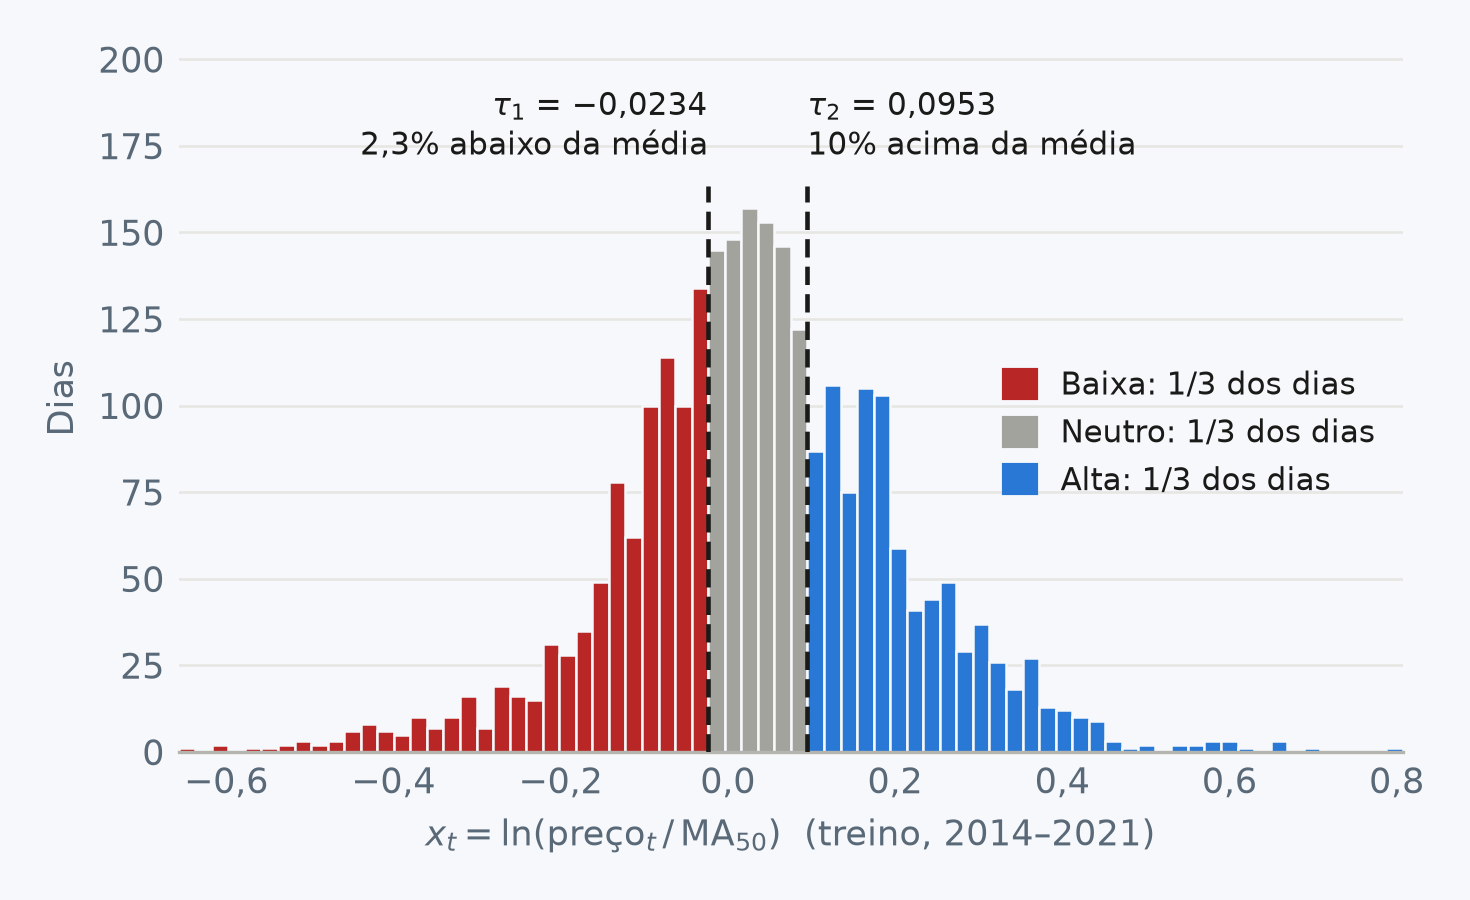
\includegraphics[width=\linewidth,height=5.2cm,keepaspectratio]{limiares_tercis.png}
        \end{altura}
      \end{block}
    \end{column}

    \begin{column}{0.32\textwidth}
      \begin{block}{Passo a passo}
        \begin{altura}{5.3cm}
        \footnotesize
        \begin{enumerate}\setlength{\itemsep}{5pt}
          \item Calcula $x_t$ em cada dia do treino
          \item Ordena do menor para o maior
          \item Corta em 3 partes iguais:
            \begin{itemize}\setlength{\itemsep}{2pt}
              \item $\tau_1$: percentil 33\%
              \item $\tau_2$: percentil 67\%
            \end{itemize}
          \item Teste usa os mesmos $\tau_1$ e $\tau_2$
        \end{enumerate}
        \vskip 6pt
        \begin{itemize}
          \item \textbf{Não simétrico:} no treino o BTC ficou mais tempo acima da média
        \end{itemize}
        \end{altura}
      \end{block}
    \end{column}
  \end{columns}

\end{frame}

% =============================================================
% SLIDE 5 — SOLUÇÃO 2: ESTIMAÇÃO EMPÍRICA DO MODELO
% =============================================================
\begin{frame}{5. Solução 2: Estimação Empírica do Modelo}

  \begin{columns}[T,onlytextwidth]
    \begin{column}{0.33\textwidth}
      \begin{block}{Transição ($\widehat{P}$)}
        \begin{altura}{1.7cm}
        \[
          \widehat{P}(s' \mid s, a) = \frac{N(s, a, s')}{N(s, a)}
        \]
        \end{altura}
      \end{block}
    \end{column}

    \begin{column}{0.63\textwidth}
      \begin{block}{Recompensa ($\widehat{R}$)}
        \begin{altura}{1.7cm}
        {\small
        \[
          \widehat{R}(s,a,s') = \frac{1}{N(s,a,s')} \sum_{k} \ln\left(1 + a \, r_{t+1}^{(k)} - \kappa |a - h_{t-1}|\right)
        \]
        }
        \end{altura}
      \end{block}
    \end{column}
  \end{columns}

  \vskip 0.1cm

  \begin{block}{$\widehat{P}$ estimada no treino (contagens de 2014 a 2021)}
    \centering\footnotesize
    \renewcommand{\arraystretch}{1.25}
    \begin{tabular}{l ccccccccc}
      \toprule
      $\big(\phi(x_t), \phi(x_{t-1})\big)$ & (0,0) & (0,1) & (0,2) & (1,0) & (1,1) & (1,2) & (2,0) & (2,1) & (2,2) \\
      \midrule
      $\phi(x_{t+1}) = 0$ & 0,933 & 0,915 & 0,333 & 0,310 & 0,053 & 0,016 & 0,000 & 0,000 & 0,000 \\
      $\phi(x_{t+1}) = 1$ & 0,065 & 0,085 & 0,333 & 0,690 & 0,889 & 0,672 & 1,000 & 0,333 & 0,052 \\
      $\phi(x_{t+1}) = 2$ & 0,001 & 0,000 & 0,333 & 0,000 & 0,057 & 0,312 & 0,000 & 0,667 & 0,948 \\
      \bottomrule
    \end{tabular}
  \end{block}

\end{frame}

% =============================================================
% SLIDE 6 — VALUE ITERATION E POLÍTICA ÓTIMA
% =============================================================
\begin{frame}{6. \textit{Value Iteration} e Política Ótima}

  \begin{block}{Equação de Otimalidade de Bellman}
    {\centering $\displaystyle V_{k+1}(s) = \max_{a} \sum_{s'} \widehat{P}(s' \mid s, a) \Big( \widehat{R}(s, a, s') + \gamma V_k(s') \Big)$\par}
    {\centering\scriptsize Convergência em \textbf{98 iterações} ($\text{tol} < 10^{-12}$, $\gamma = 0{,}8$)\par}
  \end{block}

  \vskip -0.15cm

  \begin{columns}[T,onlytextwidth]
    \begin{column}{0.64\textwidth}
      \begin{block}{Política ótima $\pi^*(s) = \arg\max_{a} Q^*(s,a)$}
        \begin{altura}{3.7cm}
        \centering\scriptsize
        \setlength{\tabcolsep}{4.5pt}
        \renewcommand{\arraystretch}{0.95}
        \begin{tabular}{c l ccc}
          \toprule
          $\big(\phi(x_t),\phi(x_{t-1})\big)$ & \textbf{Regime} & $h_{t-1}=-1$ & $h_{t-1}=0$ & $h_{t-1}=+1$ \\
          \midrule
          (0,0) & Baixa estável      & $0$  & $0$  & $+1$ \\
          (0,1) & Neutro $\to$ Baixa & $-1$ & $-1$ & $-1$ \\
          (0,2) & Alta $\to$ Baixa   & $-1$ & $0$  & $+1$ \\
          \midrule
          (1,0) & Baixa $\to$ Neutro & $-1$ & $0$  & $0$  \\
          (1,1) & Neutro estável     & $0$  & $0$  & $+1$ \\
          (1,2) & Alta $\to$ Neutro  & $+1$ & $+1$ & $+1$ \\
          \midrule
          (2,0) & Baixa $\to$ Alta   & $-1$ & $-1$ & $-1$ \\
          (2,1) & Neutro $\to$ Alta  & $+1$ & $+1$ & $+1$ \\
          (2,2) & Alta estável       & $+1$ & $+1$ & $+1$ \\
          \bottomrule
        \end{tabular}
        \end{altura}
      \end{block}
    \end{column}

    \begin{column}{0.32\textwidth}
      \begin{block}{Leitura}
        \begin{altura}{3.7cm}
        \footnotesize
        \begin{itemize}\setlength{\itemsep}{3pt}
          \item \textbf{Baixa estável:} fica fora
          \item \textbf{Entrando na baixa:} vende
          \item \textbf{Neutro:} só mantém o \textit{long}
          \item \textbf{Alta:} compra
        \end{itemize}
        \end{altura}
      \end{block}
    \end{column}
  \end{columns}

\end{frame}

% #############################################################
% PARTE III — SOLUÇÕES MODEL-FREE: MONTE CARLO E Q-LEARNING
% #############################################################

% =============================================================
% SLIDE 7 — MONTE CARLO: ALGORITMO E FIRST x EVERY-VISIT
% =============================================================
\begin{frame}{7. Monte Carlo (\textit{Model-Free})}

  \begin{columns}[T,onlytextwidth]
    \begin{column}{0.58\textwidth}
      \begin{block}{Algoritmo}
        \begin{altura}{2.25cm}
        \small
        \begin{enumerate}\setlength{\itemsep}{3pt}
          \item Episódio com retornos reais do treino
          \item Retorno: $G_t = R_{t+1} + \gamma\, G_{t+1}$
          \item Atualização: $Q(s,a) \leftarrow Q(s,a) + \tfrac{1}{N(s,a)}\big[G_t - Q(s,a)\big]$
          \item Política: $\pi(s) = \arg\max_a Q(s,a)$
        \end{enumerate}
        \end{altura}
      \end{block}
    \end{column}

    \begin{column}{0.38\textwidth}
      \begin{block}{Configuração}
        \begin{altura}{2.25cm}
        \small
        \begin{itemize}\setlength{\itemsep}{3pt}
          \item 30.000 episódios de 84 dias
          \item $\varepsilon$-greedy: $\varepsilon$ de $1$ a $0{,}05$
          \item \textit{Exploring starts}
        \end{itemize}
        \end{altura}
      \end{block}
    \end{column}
  \end{columns}

  \vskip 0.2cm

  \begin{columns}[T,onlytextwidth]
    \begin{column}{0.58\textwidth}
      \begin{block}{First-visit $\times$ Every-visit (treino, semente 42)}
        \begin{altura}{2.5cm}
        \centering\footnotesize
        \renewcommand{\arraystretch}{1.15}
        \begin{tabular}{l cc}
          \toprule
          & \textbf{First-visit} & \textbf{Every-visit} \\
          \midrule
          Passagens usadas      & só a primeira & todas \\
          Atualizações de $Q$   & 388.071       & 1.260.000 \\
          Sharpe no treino      & 1,12          & \textbf{1,20} \\
          \bottomrule
        \end{tabular}
        \end{altura}
      \end{block}
    \end{column}

    \begin{column}{0.38\textwidth}
      \begin{alertblock}{Escolha}
        \begin{altura}{2.5cm}
        \centering
        Maior Sharpe no treino
        \vskip 0.15cm
        $\Downarrow$
        \vskip 0.15cm
        \textbf{every-visit}
        \end{altura}
      \end{alertblock}
    \end{column}
  \end{columns}

\end{frame}

% =============================================================
% SLIDE 8 — Q-LEARNING E COMPARAÇÃO DOS MÉTODOS
% =============================================================
\begin{frame}{8. Q-learning e Comparação dos Métodos}

  \begin{block}{Q-learning: atualiza a cada passo (\textit{bootstrap}), mesmos episódios do MC}
    \[
      Q(s,a) \leftarrow Q(s,a) + \frac{1}{N(s,a)}\Big[\underbrace{R_{t+1} + \gamma \max_{a'} Q(s',a')}_{\text{alvo}} - Q(s,a)\Big]
    \]
  \end{block}

  \vskip 0.1cm

  \begin{block}{\textit{Value Iteration} $\times$ Monte Carlo $\times$ Q-learning}
    \centering\scriptsize
    \setlength{\tabcolsep}{6pt}
    \renewcommand{\arraystretch}{1.0}
    \begin{tabular}{l ccc}
      \toprule
      & \textbf{\textit{Value Iteration}} & \textbf{Monte Carlo} & \textbf{Q-learning} \\
      \midrule
      Precisa do modelo?       & sim ($\widehat{P}$, $\widehat{R}$)                          & não                       & não \\
      Alvo da atualização      & $\sum_{s'} \widehat{P}\,\big[\widehat{R} + \gamma V(s')\big]$ & retorno real $G_t$        & $R_{t+1} + \gamma \max_{a'} Q(s',a')$ \\
      Quando atualiza          & todos os estados, a cada iteração                         & no fim do episódio        & a cada passo \\
      Supõe Markov?            & sim                                                       & não                       & sim \\
      Aprende                  & --                                                        & \textit{on-policy}        & \textit{off-policy} \\
      \midrule
      Custo do treino          & 98 iterações                                              & 1.260.000 atualizações    & 2.520.000 atualizações \\
      Sharpe no treino         & 1,09                                                      & 1,20                      & 1,37 \\
      \bottomrule
    \end{tabular}
  \end{block}

\end{frame}

% =============================================================
% SLIDE 9 — POLÍTICA APRENDIDA PELOS TRÊS MÉTODOS
% =============================================================
\begin{frame}{9. Política Aprendida pelos Três Métodos}

  \begin{columns}[T,onlytextwidth]
    \begin{column}{0.66\textwidth}
      \begin{block}{Ação por estado (vermelho: os métodos discordam)}
        \begin{altura}{4.5cm}
        \centering\scriptsize
        \setlength{\tabcolsep}{3pt}
        \renewcommand{\arraystretch}{1.1}
        \begin{tabular}{c l ccc ccc ccc}
          \toprule
          & & \multicolumn{3}{c}{\textbf{VI} ($h_{t-1}$)} & \multicolumn{3}{c}{\textbf{MC} ($h_{t-1}$)} & \multicolumn{3}{c}{\textbf{QL} ($h_{t-1}$)} \\
          \cmidrule(lr){3-5} \cmidrule(lr){6-8} \cmidrule(lr){9-11}
          \textbf{Estado} & \textbf{Regime} & $-1$ & $0$ & $+1$ & $-1$ & $0$ & $+1$ & $-1$ & $0$ & $+1$ \\
          \midrule
          (0,0) & Baixa estável        & $0$ & $0$ & $+1$ & $0$ & $0$ & $+1$ & $0$ & $0$ & $+1$ \\
          (0,1) & Neutro $\to$ Baixa   & $-1$ & $-1$ & $\dif{-1}$ & $-1$ & $-1$ & $\dif{0}$ & $-1$ & $-1$ & $\dif{0}$ \\
          (0,2) & Alta $\to$ Baixa     & $\dif{-1}$ & $0$ & $\dif{+1}$ & $\dif{0}$ & $0$ & $\dif{0}$ & $\dif{0}$ & $0$ & $\dif{0}$ \\
          \midrule
          (1,0) & Baixa $\to$ Neutro   & $\dif{-1}$ & $\dif{0}$ & $\dif{0}$ & $\dif{0}$ & $\dif{0}$ & $\dif{-1}$ & $\dif{0}$ & $\dif{-1}$ & $\dif{0}$ \\
          (1,1) & Neutro estável       & $0$ & $\dif{0}$ & $+1$ & $0$ & $\dif{0}$ & $+1$ & $0$ & $\dif{+1}$ & $+1$ \\
          (1,2) & Alta $\to$ Neutro    & $+1$ & $+1$ & $+1$ & $+1$ & $+1$ & $+1$ & $+1$ & $+1$ & $+1$ \\
          \midrule
          (2,0) & Baixa $\to$ Alta     & $-1$ & $-1$ & $-1$ & $-1$ & $-1$ & $-1$ & $-1$ & $-1$ & $-1$ \\
          (2,1) & Neutro $\to$ Alta    & $+1$ & $+1$ & $+1$ & $+1$ & $+1$ & $+1$ & $+1$ & $+1$ & $+1$ \\
          (2,2) & Alta estável         & $+1$ & $+1$ & $+1$ & $+1$ & $+1$ & $+1$ & $+1$ & $+1$ & $+1$ \\
          \bottomrule
        \end{tabular}
        \end{altura}
      \end{block}
    \end{column}

    \begin{column}{0.30\textwidth}
      \begin{block}{Leitura}
        \begin{altura}{4.5cm}
        \footnotesize
        \begin{itemize}\setlength{\itemsep}{3pt}
          \item Os três iguais em \textbf{20/27} estados
          \item MC e QL: 24/27 iguais
          \item Alta: mesma ação nos três
          \item Diferenças perto da baixa e no neutro
          \item $(0,2)$ nunca ocorre no treino
        \end{itemize}
        \end{altura}
      \end{block}
    \end{column}
  \end{columns}

\end{frame}

% =============================================================
% SLIDE 10 — CURVAS DE APRENDIZADO (5 SEMENTES)
% =============================================================
\begin{frame}{10. Convergência: Monte Carlo $\times$ Q-learning}

  \centering
  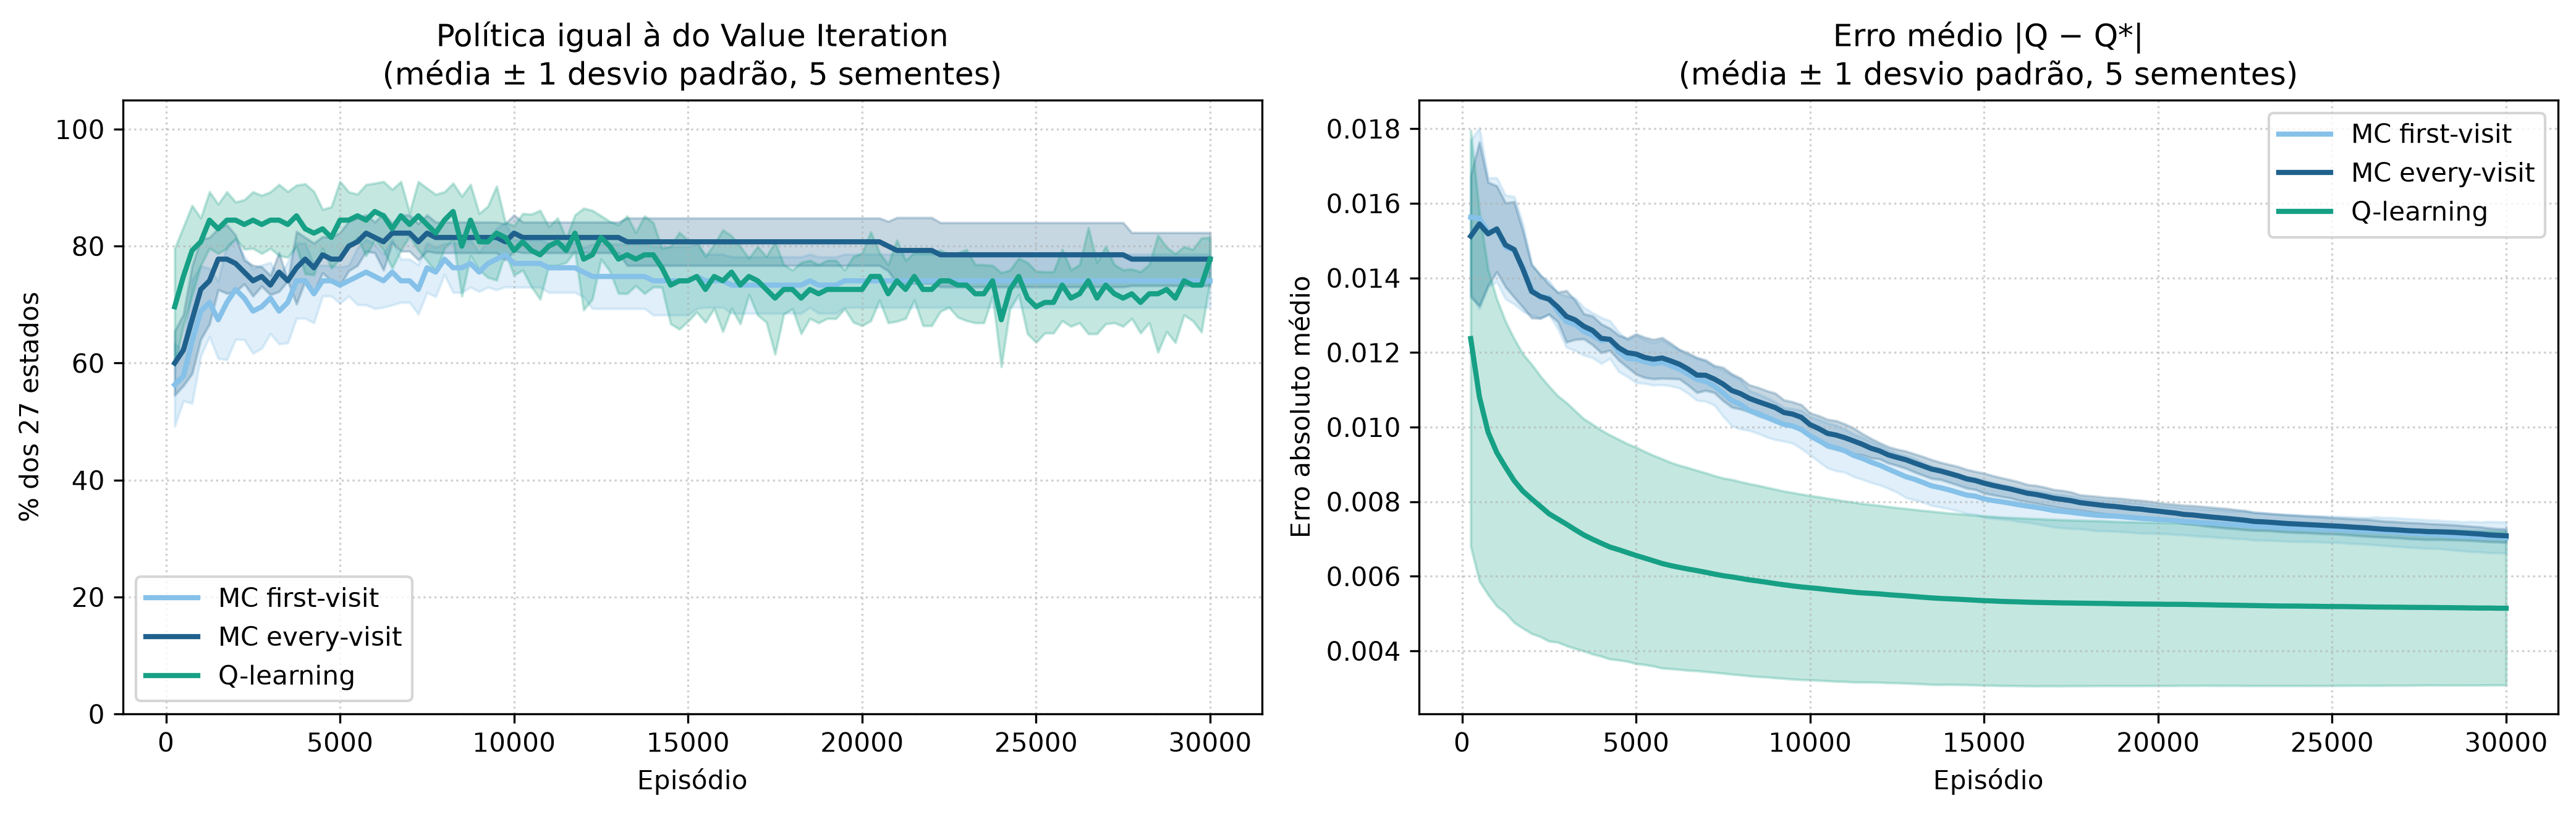
\includegraphics[width=0.94\textwidth]{curva_sementes.png}

  \vskip 0.1cm
  \raggedright\small
  \begin{itemize}\setlength{\itemsep}{2pt}
    \item Referência teórica: $Q^*$ do VI, mesmo MDP
    \item Q-learning chega mais perto de $Q^*$: erro 0,005 (MC: 0,007)
    \item Mas varia mais entre as 5 sementes
  \end{itemize}

\end{frame}

% =============================================================
% SLIDE 11 — MONTE CARLO E Q-LEARNING COM 5 SEMENTES
% =============================================================
\begin{frame}{11. Monte Carlo e Q-learning com 5 Sementes}

  \begin{block}{5 treinos de 30.000 episódios, cada um com sorteios diferentes (sementes 42 a 46)}
    \centering\scriptsize
    \setlength{\tabcolsep}{7pt}
    \renewcommand{\arraystretch}{1.05}
    \begin{tabular}{ll c ccc}
      \toprule
      & & \textbf{Treino} & \multicolumn{3}{c}{\textbf{Teste (2022 a 2026)}} \\
      \cmidrule(lr){3-3} \cmidrule(lr){4-6}
      \textbf{Método} & & \textbf{Sharpe} & \textbf{Sharpe} & \textbf{Max Drawdown} & \textbf{Calmar} \\
      \midrule
      MC first-visit & Média         & 1,42   & 0,30   & -39,07\% & 0,44   \\
                     & Desvio padrão & 0,17   & 0,26   & 19,31\%  & 0,39   \\
                     & Variância     & 0,0291 & 0,0680 & 0,0373   & 0,1486 \\
      \midrule
      MC every-visit & Média         & 1,17            & 0,34            & -33,24\%         & 0,47   \\
                     & Desvio padrão & \textbf{0,04}   & \textbf{0,09}   & \textbf{7,94\%}  & 0,17   \\
                     & Variância     & \textbf{0,0015} & \textbf{0,0077} & \textbf{0,0063}  & 0,0301 \\
      \midrule
      Q-learning     & Média         & 1,31   & 0,24   & -49,58\% & 0,27            \\
                     & Desvio padrão & 0,10   & 0,12   & 13,24\%  & \textbf{0,12}   \\
                     & Variância     & 0,0098 & 0,0155 & 0,0175   & \textbf{0,0143} \\
      \bottomrule
    \end{tabular}
  \end{block}

  \small
  \begin{itemize}\setlength{\itemsep}{2pt}
    \item Every-visit: o mais estável (menor desvio no teste)
    \item Q-learning: mesma ação em 21/27 estados nas 5 sementes
    \item Na média, o first-visit vence no treino: com 1 semente, a escolha dependeu da sorte
  \end{itemize}

\end{frame}

% #############################################################
% PARTE IV — AVALIAÇÃO NO TESTE
% #############################################################

% =============================================================
% SLIDE 12 — MÉTRICAS DE AVALIAÇÃO
% =============================================================
\begin{frame}{12. Métricas de Avaliação}

  \begin{block}{Métricas de risco e retorno}
    \centering\small
    \setlength{\tabcolsep}{10pt}
    \begin{tabular}{l c l}
      \toprule
      \textbf{Métrica} & \textbf{Fórmula} & \textbf{O que mede} \\
      \midrule
      \addlinespace[5pt]
      Índice de Sharpe   & $\displaystyle \sqrt{365}\;\frac{\bar e}{\sigma_e}$    & retorno extra por unidade de volatilidade \\
      \addlinespace[9pt]
      Maximum Drawdown   & $\displaystyle \min_t \Big(\frac{W_t}{P_t} - 1\Big)$ & maior queda percentual do patrimônio \\
      \addlinespace[9pt]
      Índice de Calmar   & $\displaystyle \frac{R_{\text{anual}}}{|\text{MDD}|}$ & retorno anual por unidade de queda máxima \\
      \addlinespace[5pt]
      \bottomrule
    \end{tabular}
  \end{block}

  \footnotesize
  \begin{itemize}\setlength{\itemsep}{2pt}
    \item $W_t$: patrimônio no dia $t$ \qquad $P_t$: maior patrimônio até $t$
    \item $e_t$: retorno diário acima da taxa livre de risco (T-bill de 3 meses)
    \item 1 ano $=$ 365 dias
  \end{itemize}

\end{frame}

% =============================================================
% SLIDE 13 — RESULTADOS NO SIMULADOR
% =============================================================
\begin{frame}{13. Resultados no \texttt{gym-trading-env}}

  \begin{block}{BTC-USD, $\kappa = 0{,}1\%$, $\gamma = 0{,}8$}
    \centering\scriptsize
    \setlength{\tabcolsep}{5pt}
    \renewcommand{\arraystretch}{1.05}
    \begin{tabular}{l cccccc}
      \toprule
      \textbf{Estratégia} & \textbf{Retorno Total} & \textbf{Retorno Anual} & \textbf{Sharpe} & \textbf{Max Drawdown} & \textbf{Calmar} & \textbf{Trocas} \\
      \midrule
      \multicolumn{7}{l}{\textit{Teste (2022 a 2026)}} \\
      MDP (Value Iteration)          & 127,80\%          & 18,37\%          & 0,46          & -29,35\%          & 0,63          & 113 \\
      Monte Carlo (every-visit)      & 119,47\%          & 17,47\%          & 0,44          & -26,95\%          & 0,65          & 108 \\
      Q-learning                     & 86,39\%           & 13,60\%          & 0,26          & -51,25\%          & 0,27          & 190 \\
      Buy \& Hold                    & 31,95\%           & 5,84\%           & 0,04          & -66,93\%          & 0,09          & 1 \\
      Fora do Mercado                & 0,00\%            & 0,00\%           & 0,00          & 0,00\%            & --            & 0 \\
      Aleatória                      & -93,85\%          & -43,52\%         & -1,45         & -94,58\%          & -0,46         & 1.163 \\
      \midrule
      \multicolumn{7}{l}{\textit{Treino (2014 a 2021)}} \\
      MDP (Value Iteration)          & 6.947,44\%        & 81,24\%          & 1,09          & -50,59\%          & 1,61          & 140 \\
      Monte Carlo (every-visit)      & 9.802,30\%        & 90,06\%          & 1,20          & -52,95\%          & 1,70          & 119 \\
      Q-learning                     & 26.866,84\%       & 118,62\%         & 1,37          & -69,05\%          & 1,72          & 195 \\
      Buy \& Hold                    & 13.144,05\%       & 97,94\%          & 0,90          & -83,40\%          & 1,17          & 1 \\
      Fora do Mercado                & 0,00\%            & 0,00\%           & 0,00          & 0,00\%            & --            & 0 \\
      Aleatória                      & -88,73\%          & -26,29\%         & -0,52         & -95,74\%          & -0,27         & 1.721 \\
      \bottomrule
    \end{tabular}
  \end{block}

\end{frame}

% =============================================================
% SLIDE 14 — COM E SEM CORRETAGEM
% =============================================================
\begin{frame}{14. Com e Sem Corretagem no Teste}

  \begin{block}{Mesmas políticas no teste (2022 a 2026), com e sem corretagem}
    \centering\scriptsize
    \setlength{\tabcolsep}{5pt}
    \renewcommand{\arraystretch}{1.0}
    \begin{tabular}{l cccccc}
      \toprule
      \textbf{Estratégia} & \textbf{Retorno Total} & \textbf{Retorno Anual} & \textbf{Sharpe} & \textbf{Max Drawdown} & \textbf{Calmar} & \textbf{Trocas} \\
      \midrule
      \multicolumn{7}{l}{\textit{Com corretagem ($\kappa = 0{,}1\%$ por troca)}} \\
      MDP (Value Iteration)      & 127,80\%  & 18,37\%  & 0,46  & -29,35\%  & 0,63  & 113 \\
      Monte Carlo (every-visit)  & 119,47\%  & 17,47\%  & 0,44  & -26,95\%  & 0,65  & 108 \\
      Q-learning                 & 86,39\%   & 13,60\%  & 0,26  & -51,25\%  & 0,27  & 190 \\
      Buy \& Hold                & 31,95\%   & 5,84\%   & 0,04  & -66,93\%  & 0,09  & 1 \\
      Aleatória                  & -93,85\%  & -43,52\% & -1,45 & -94,58\%  & -0,46 & 1.163 \\
      \midrule
      \multicolumn{7}{l}{\textit{Sem corretagem ($\kappa = 0$)}} \\
      MDP (Value Iteration)      & 158,32\%  & 21,46\%  & 0,55  & -28,42\%  & 0,75  & 113 \\
      Monte Carlo (every-visit)  & 144,45\%  & 20,09\%  & 0,51  & -26,29\%  & 0,76  & 108 \\
      Q-learning                 & 125,43\%  & 18,12\%  & 0,37  & -48,39\%  & 0,37  & 190 \\
      Buy \& Hold                & 32,09\%   & 5,87\%   & 0,04  & -66,89\%  & 0,09  & 1 \\
      Aleatória                  & -70,23\%  & -21,98\% & -0,68 & -74,63\%  & -0,29 & 1.163 \\
      \bottomrule
    \end{tabular}
  \end{block}

  \small
  \begin{itemize}\setlength{\itemsep}{2pt}
    \item Mesmas ações: a diferença é só o custo das trocas
    \item Quem troca mais paga mais: Q-learning perde 4,5 p.p. ao ano
    \item A ordem entre as estratégias não muda
  \end{itemize}

\end{frame}

% =============================================================
% SLIDE 15 — DESEMPENHO NO TESTE (GRÁFICO)
% =============================================================
\begin{frame}{15. Desempenho no Período de Teste}
  \centering
  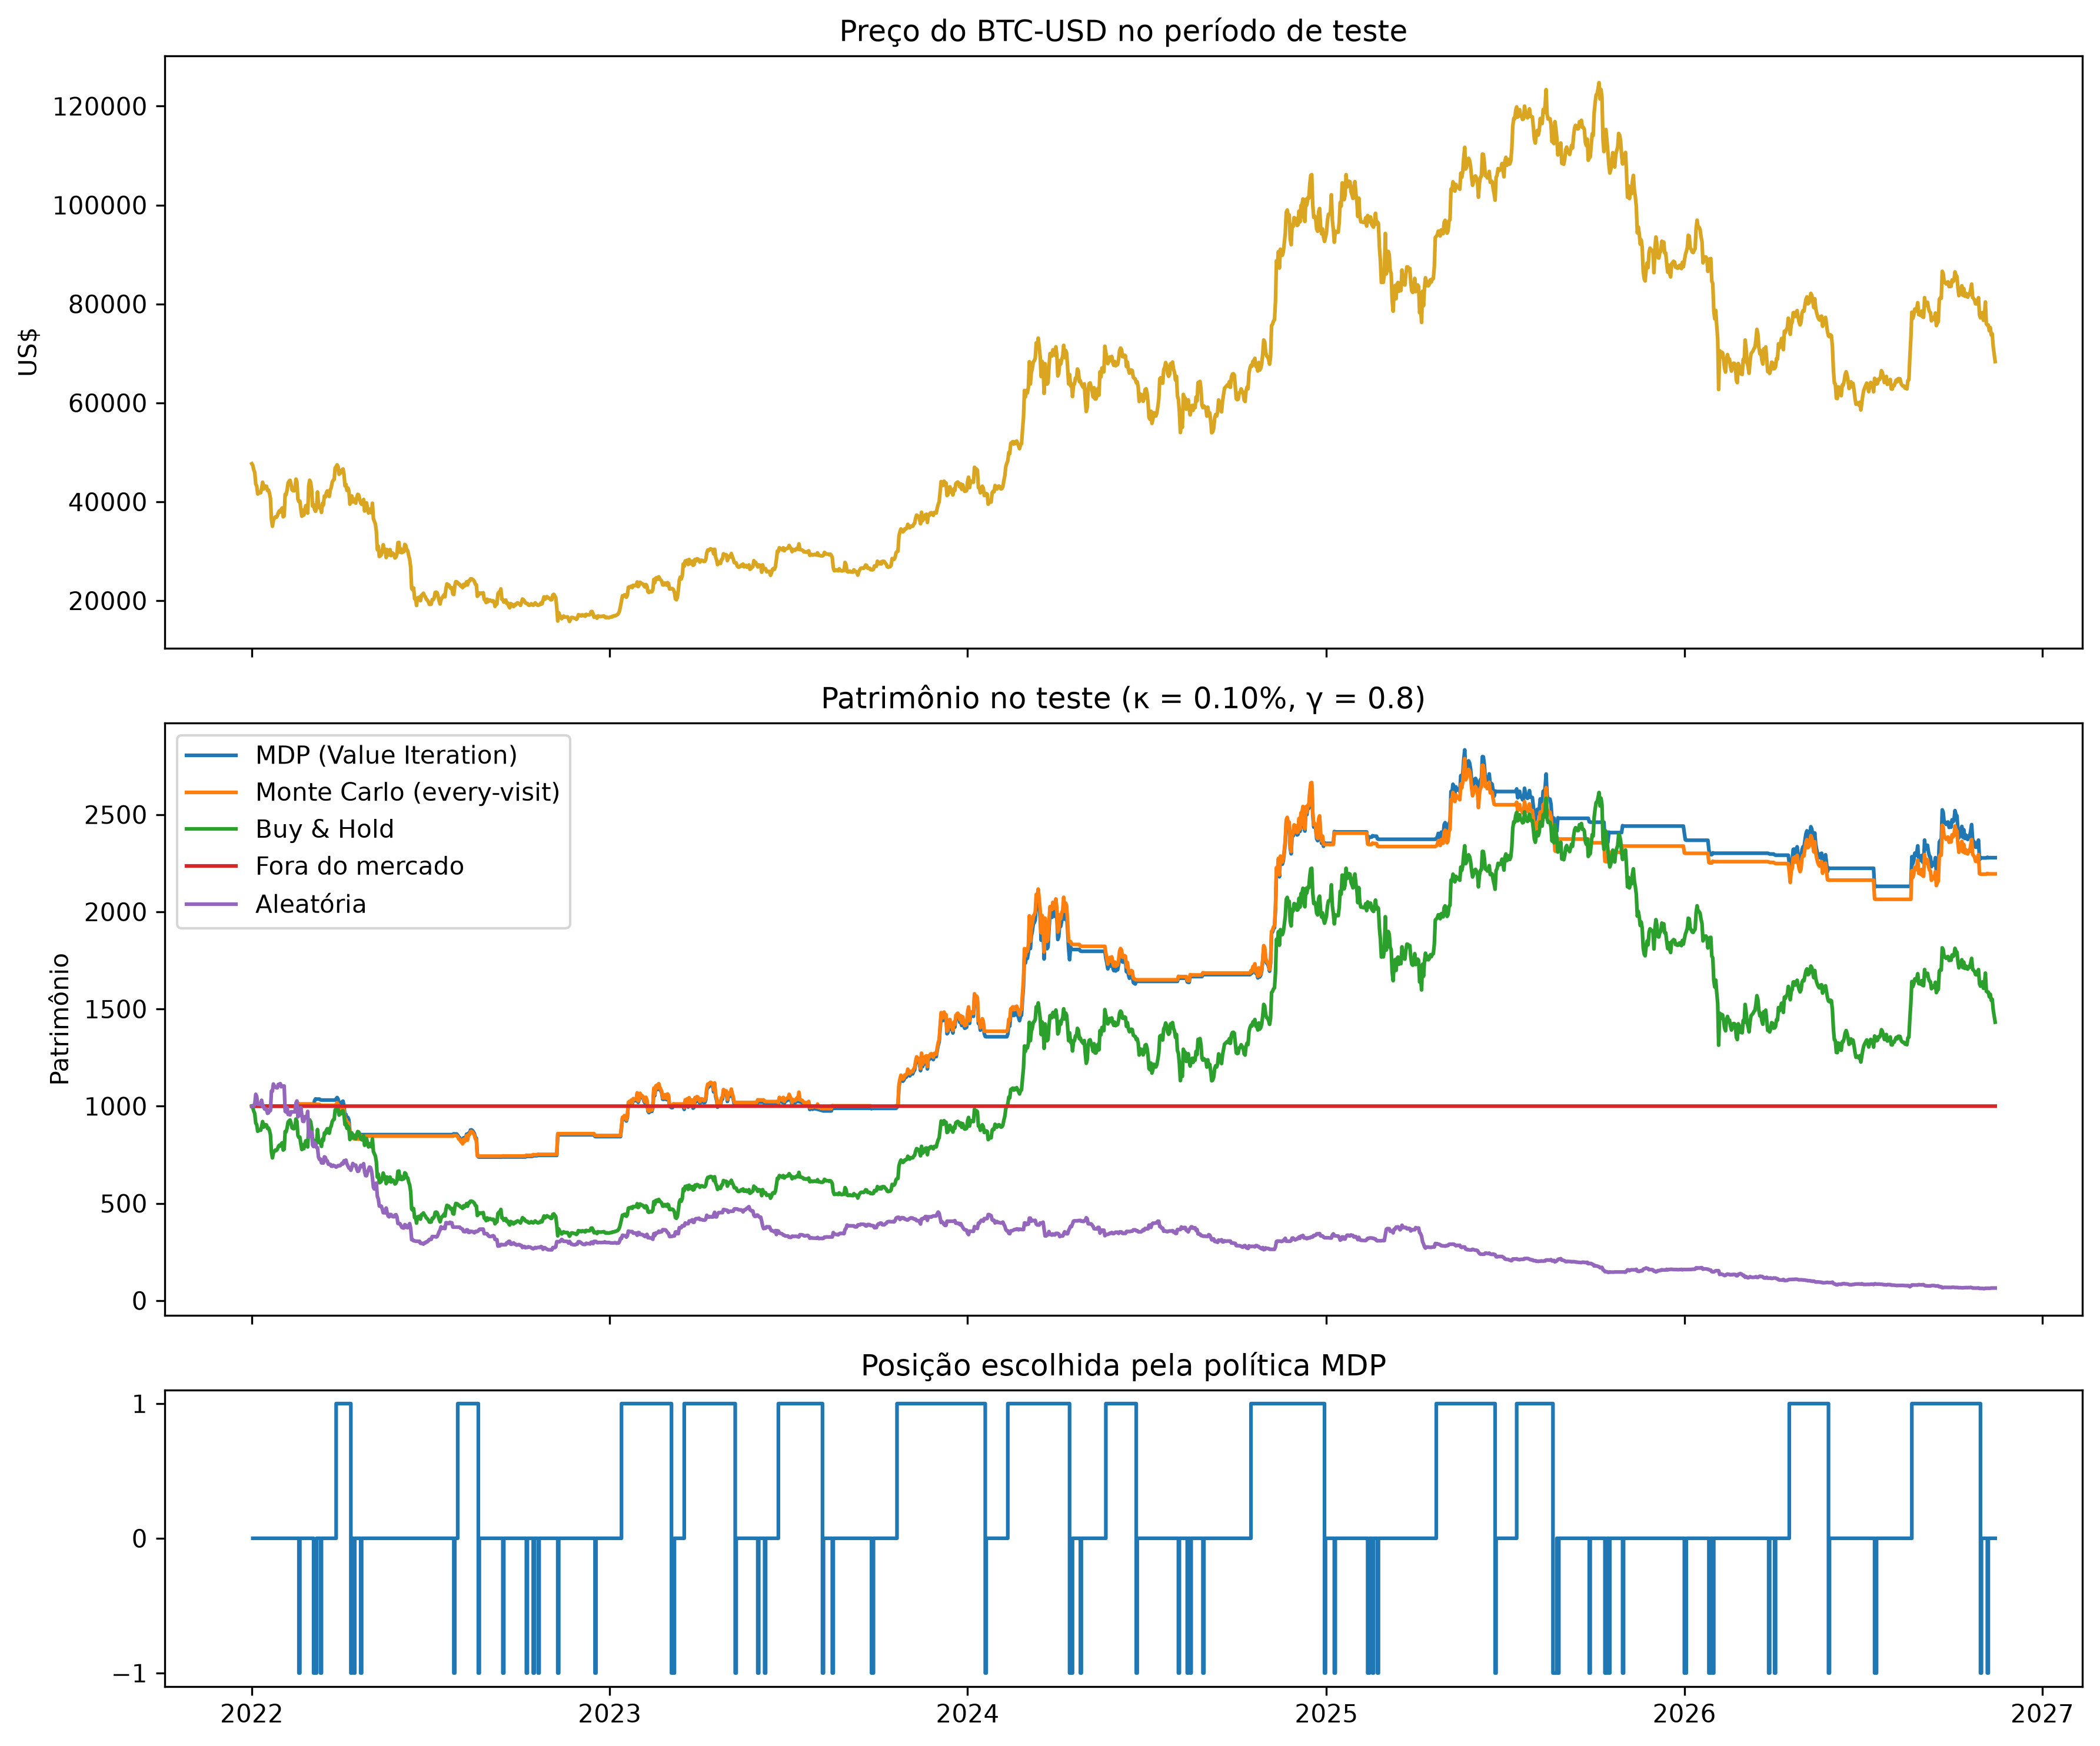
\includegraphics[height=0.86\textheight]{grafico_teste.png}
\end{frame}

% =============================================================
% SLIDE 16 — POLÍTICA GULOSA x EPSILON-GREEDY
% =============================================================
\begin{frame}{16. Política Gulosa $\times$ $\varepsilon$-greedy}

  \begin{columns}[T,onlytextwidth]
    \begin{column}{0.48\textwidth}
      \begin{block}{Gulosa}
        {\centering $\displaystyle a_t = \arg\max_a Q(s_t, a)$\par}
        \vskip 3pt
        {\centering\footnotesize sempre a ação de maior valor\par}
      \end{block}
    \end{column}

    \begin{column}{0.48\textwidth}
      \begin{block}{$\varepsilon$-greedy ($\varepsilon = 0{,}1$)}
        {\centering $\displaystyle \pi(a^* \mid s) = 1 - \varepsilon + \varepsilon/3$\par}
        \vskip 3pt
        {\centering\footnotesize com probabilidade $\varepsilon$, a ação é sorteada\par}
      \end{block}
    \end{column}
  \end{columns}

  \vskip 0.1cm

  \begin{block}{Teste (2022 a 2026) \quad $\varepsilon$-greedy: média de 100 sementes}
    \centering\scriptsize
    \setlength{\tabcolsep}{7pt}
    \renewcommand{\arraystretch}{1.0}
    \begin{tabular}{l ccccc}
      \toprule
      \textbf{Política} & \textbf{Sharpe} & \textbf{Max Drawdown} & \textbf{Calmar} & \textbf{Trocas} & \textbf{$\varepsilon >$ gulosa (\% sementes)} \\
      \midrule
      \textbf{MDP: gulosa}                    & \textbf{0,46} & \textbf{-29,35\%} & \textbf{0,63} & \textbf{113} & --          \\
      MDP: $\varepsilon$-greedy               & 0,20          & -49,87\%          & 0,29          & 286          & 24\%        \\
      \midrule
      \textbf{Monte Carlo: gulosa}            & \textbf{0,44} & \textbf{-26,95\%} & \textbf{0,65} & \textbf{108} & --          \\
      Monte Carlo: $\varepsilon$-greedy       & 0,14          & -50,67\%          & 0,24          & 289          & 21\%        \\
      \midrule
      \textbf{Q-learning: gulosa}             & \textbf{0,26} & \textbf{-51,25\%} & \textbf{0,27} & \textbf{190} & --          \\
      Q-learning: $\varepsilon$-greedy        & 0,04          & -59,22\%          & 0,13          & 373          & 23\%        \\
      \bottomrule
    \end{tabular}
  \end{block}

  \small
  \begin{itemize}\setlength{\itemsep}{2pt}
    \item A gulosa vence nos três métodos
    \item Explorar serve para aprender, não para operar
  \end{itemize}

\end{frame}

% =============================================================
% SLIDE 17 — BENCHMARK: RL VS MODELOS ECONOMÉTRICOS
% =============================================================
\begin{frame}{17. Benchmark no Teste: RL $\times$ Modelos Econométricos}

  \begin{block}{Ranking por Sharpe \quad (Calmar = retorno anual / $|$max drawdown$|$)}
    \centering\footnotesize
    \setlength{\tabcolsep}{7pt}
    \renewcommand{\arraystretch}{1.05}
    \begin{tabular}{l ccccc}
      \toprule
      \textbf{Modelo} & \textbf{Retorno Total} & \textbf{Sharpe} & \textbf{Max Drawdown} & \textbf{Calmar} & \textbf{Trocas} \\
      \midrule
      \textbf{MDP (Value Iteration)}   & \textbf{+126,86\%} & \textbf{0,46} & \textbf{-29,35\%} & \textbf{0,62} & \textbf{113} \\
      \textbf{Monte Carlo}             & \textbf{+119,46\%} & \textbf{0,44} & \textbf{-26,95\%} & \textbf{0,65} & \textbf{108} \\
      \textbf{Q-learning}              & \textbf{+86,08\%}  & \textbf{0,26} & \textbf{-51,28\%} & \textbf{0,26} & \textbf{190} \\
      \midrule
      AR(1)                            & +110,82\% & 0,23  & -73,07\% & 0,23  & 49  \\
      ARMA(1,1)                        & +100,18\% & 0,21  & -72,85\% & 0,21  & 43  \\
      Probit                           & +54,51\%  & 0,10  & -72,95\% & 0,13  & 113 \\
      Logit                            & +50,53\%  & 0,09  & -72,95\% & 0,12  & 115 \\
      Buy \& Hold (passeio aleatório)  & +31,95\%  & 0,04  & -66,93\% & 0,09  & 1   \\
      Markov-switching (Hamilton)      & +31,95\%  & 0,04  & -66,93\% & 0,09  & 1   \\
      Regressão preditiva (OLS)        & -48,48\%  & -0,35 & -77,59\% & -0,16 & 225 \\
      \bottomrule
    \end{tabular}
  \end{block}

  \small
  \begin{itemize}\setlength{\itemsep}{2pt}
    \item RL lidera em Sharpe e Calmar
    \item MDP e MC: menos da metade da queda máxima dos econométricos
  \end{itemize}

\end{frame}

% =============================================================
% SLIDE 18 — WALK-FORWARD: A IDEIA
% =============================================================
\begin{frame}{18. Walk-forward: Retreinar ao Longo do Tempo}

  \centering
  \begin{tikzpicture}[x=1cm, y=1cm, font=\footnotesize]
    % início do teste
    \draw[dashed, SlateGray] (7.6,0.2) -- (7.6,3.4);
    \node[above, SlateGray, font=\scriptsize] at (7.6,3.4) {início do teste (jan/2022)};

    % Treino único
    \node[anchor=east, align=right] at (2.4,2.95) {\textbf{Treino único}};
    \fill[NavyDark]     (2.6,2.73) rectangle (7.6,3.17);
    \node[white] at (5.1,2.95) {treina com 2014--2021};
    \fill[SlateGray!30] (7.6,2.73) rectangle (13.6,3.17);
    \node at (10.6,2.95) {opera 2022--2026 \textbf{sem reaprender}};

    % Walk-forward (exemplo: a cada 3 meses)
    \node[anchor=east, align=right] at (2.4,1.25) {\textbf{Walk-forward}\\{\scriptsize ex.: a cada 3 meses}};
    \foreach \k/\y in {0/1.9, 1/1.25, 2/0.6} {
      \pgfmathsetmacro{\fim}{7.6+1.5*\k}
      \pgfmathsetmacro{\op}{\fim+1.5}
      \fill[NavyDark]     (2.6,\y-0.22)  rectangle (\fim,\y+0.22);
      \fill[OperaGreen]   (\fim,\y-0.22) rectangle (\op,\y+0.22);
      \fill[SlateGray!10] (\op,\y-0.22)  rectangle (13.6,\y+0.22);
      \node[white] at ({(2.6+\fim)/2},\y) {treina com tudo até aqui};
      \node[white, font=\scriptsize] at ({\fim+0.75},\y) {opera};
    }
    \node[SlateGray, font=\scriptsize] at (11.35,1.9) {futuro (não usado)};
  \end{tikzpicture}

  \vskip 0.35cm
  \begin{columns}[T,onlytextwidth]
    \begin{column}{0.48\textwidth}
      \begin{block}{Configurações testadas}
        \begin{altura}{1.1cm}
          \small
          \begin{itemize}\setlength{\itemsep}{2pt}
            \item Frequência: nunca, 3, 6 ou 12 meses
            \item Dados: todo o histórico ou últimos 4 anos
          \end{itemize}
        \end{altura}
      \end{block}
    \end{column}
    \begin{column}{0.48\textwidth}
      \begin{alertblock}{Escolha sem olhar o teste}
        \begin{altura}{1.1cm}
          \small
          \begin{itemize}\setlength{\itemsep}{2pt}
            \item Critério: maior Sharpe na validação
            \item Validação: 2019--2021, dentro do treino
          \end{itemize}
        \end{altura}
      \end{alertblock}
    \end{column}
  \end{columns}

\end{frame}

% =============================================================
% SLIDE 19 — WALK-FORWARD: RESULTADO
% =============================================================
\begin{frame}{19. Walk-forward: Resultado no Teste}

  \begin{block}{Sharpe no teste (2022 a 2026), retreinando com todo o histórico}
    \centering\small
    \setlength{\tabcolsep}{10pt}
    \renewcommand{\arraystretch}{1.12}
    \begin{tabular}{l c ccc c}
      \toprule
      & \textbf{Nunca} & \multicolumn{3}{c}{\textbf{Retreina a cada}} & \textbf{Opção escolhida} \\
      \cmidrule(lr){3-5}
      \textbf{Modelo} & \textbf{retreina} & 12 meses & 6 meses & 3 meses & \textbf{na validação} \\
      \midrule
      MDP (VI)          & 0,46          & 0,28    & 0,35    & 0,07    & nunca \\
      Monte Carlo       & 0,44          & 0,14    & 0,18    & 0,26    & 3 meses \\
      Q-learning        & 0,26          & $-$0,03 & 0,25    & $-$0,17 & 3 meses \\
      AR(1)             & 0,23          & 0,18    & 0,06    & 0,06    & 12 meses \\
      Buy \& Hold       & 0,04          & 0,04    & 0,04    & 0,04    & -- \\
      \bottomrule
    \end{tabular}
  \end{block}

  \small
  \begin{itemize}\setlength{\itemsep}{2pt}
    \item Retreinar \textbf{não melhorou nenhum modelo}
    \item MDP treinado uma vez continua o melhor
    \item Motivo: cada retreino muda tercis e probabilidades, e a política troca de ação
  \end{itemize}

\end{frame}

\end{document}
